\chapter{研究方案}
本项目分为四块内容:KITTI数据集的转换以及数据预处理,YOLO关键技术的实现,网络结构的调整与优化,测试模型的评估方法。
\section{数据预处理}{
	\subsection{KITTI数据集详解}
	\begin{figure}[htbp]
	\centering
	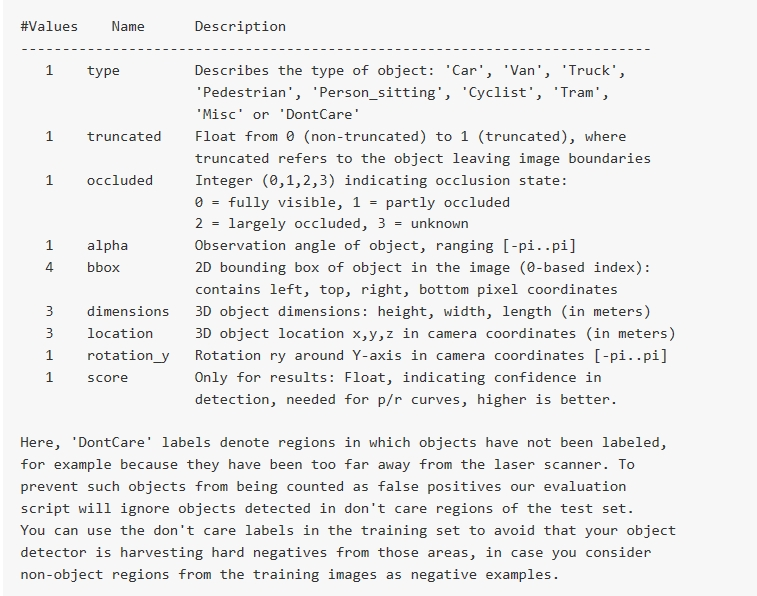
\includegraphics[width=5in]{images/KITTIForm.jpg}
	\caption{KITTI格式}
	\label{KITTIForm}
	\end{figure}
	KITTI数据集中共有7480张图片可以用来训练和测试。图\ref{KITTIForm}展示了KITTI数据集的典型样本,分为 ’Road’, ’City’, ’Residential’, ’Campus’ 和’Person’五类。原始数据采集于2011年的5天,共有180GB数据。

	\begin{figure}[htbp]
	\centering
	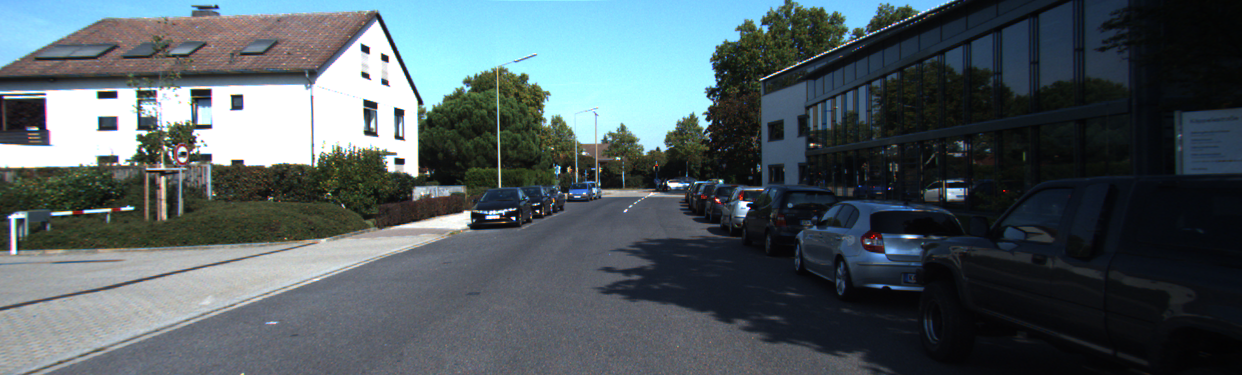
\includegraphics[width=5in]{images/007435.png}
	\caption{KITTI图像}
	\label{007435}
	\end{figure}
	数据图像如图\ref{007435},每张图片大小在1224*370左右。每张图片最多可显示15辆汽车和30名行人。

	\begin{figure}[htbp]
	\centering
	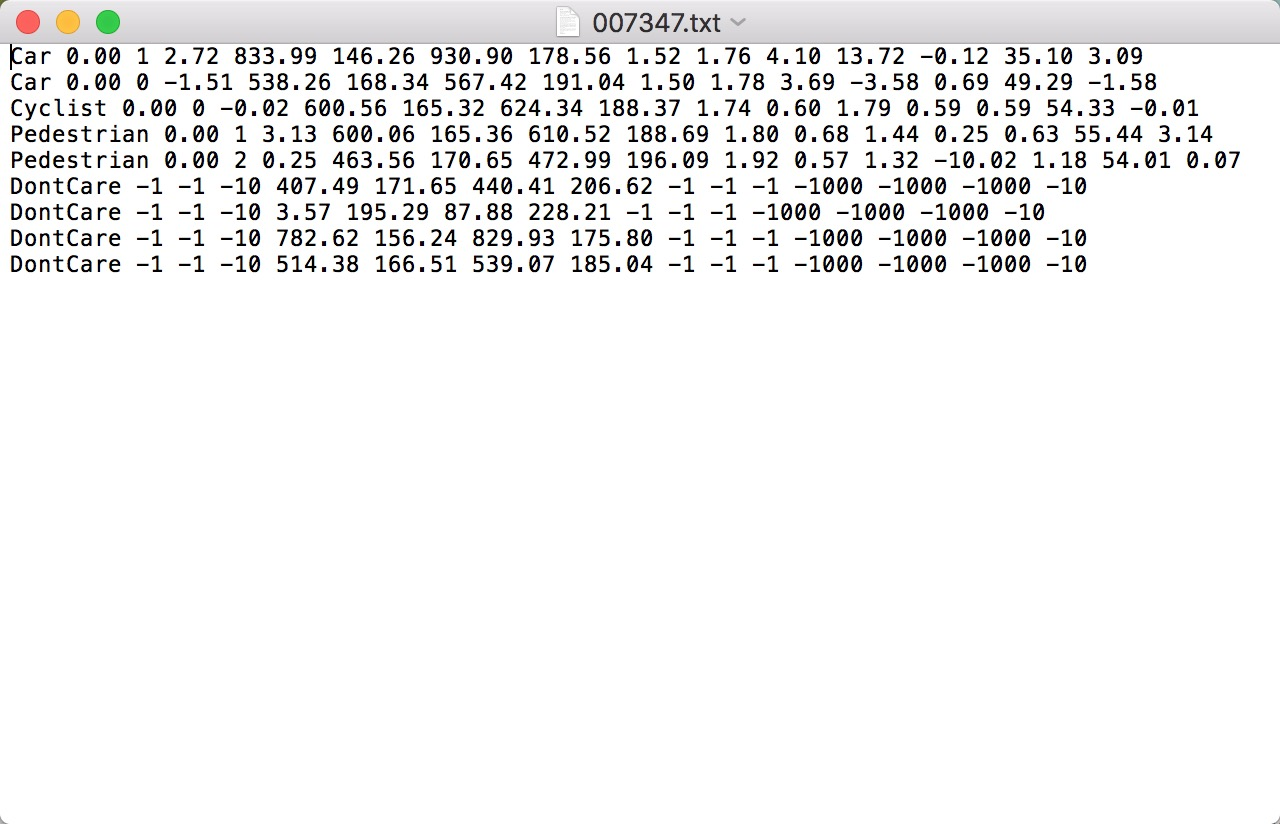
\includegraphics[width=5in]{images/KITTILable.png}
	\caption{KITTI标签}
	\label{KITTILable}
	\end{figure}
	数据标签如图\ref{KITTILable},每行是一个单独的物体。第一列是类名,而KITTI总共把所有的物体分了八个类(还有一个类名是DontCare,表示该区域没有被标注,防止假阳性);第二列代表物体超出边界多少;第三列表示物体被覆盖的情况;第四列是观察物体的角度;第五列到第八列是物体在图片中的位置(Xmin,Ymin,Xmax,Ymax);第九列到第十一列是三维物体的长宽高;第十二列到第十四列是三维物体在摄像机中的坐标(x,y,z),第十五列是物体在摄像机的坐标中离y轴的弧度。

	\subsection{数据转换和预处理}
	在实验过程中,我们将前7000张图片作为训练图片,后480张图片作为测试图片。

	\begin{figure}[htbp]
	\centering
	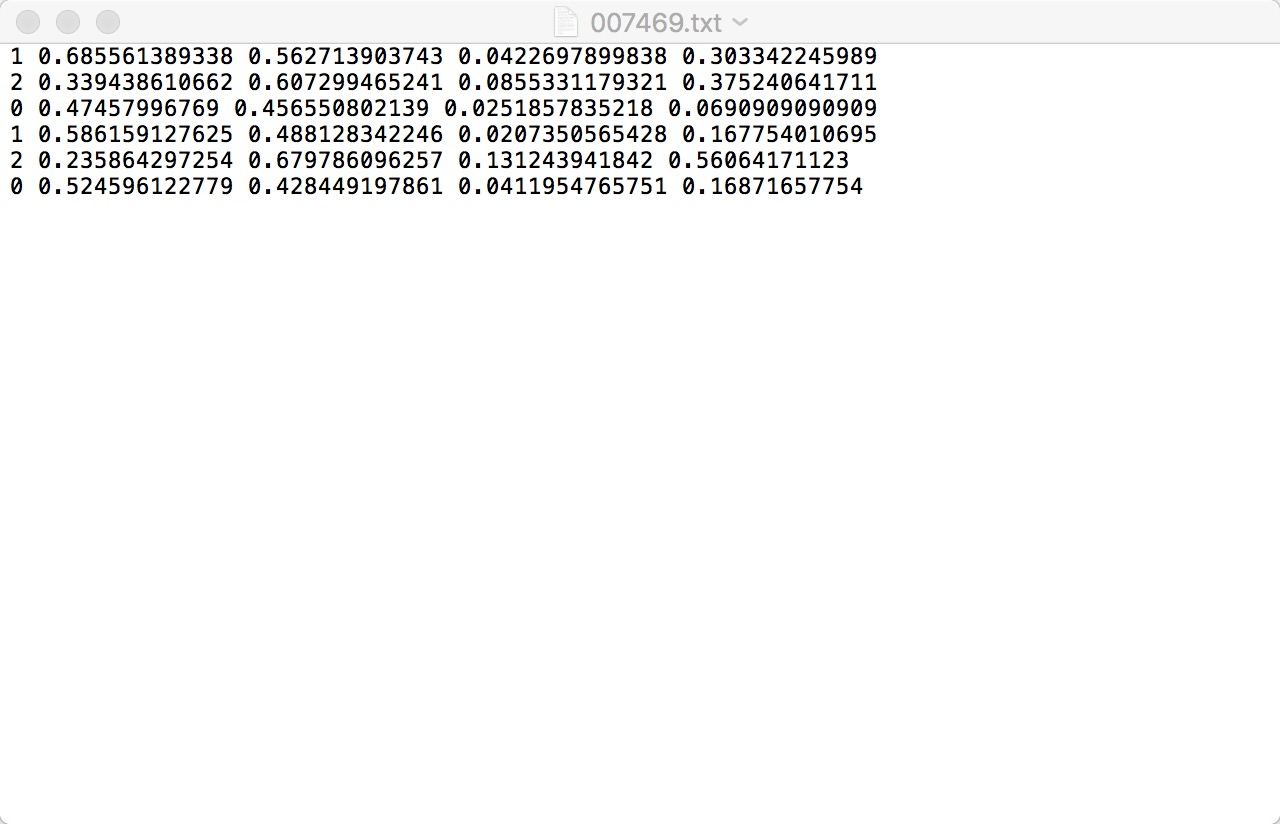
\includegraphics[width=5in]{images/darknetLabel.png}
	\caption{Darknet标签}
	\label{darknetLabel}
	\end{figure}
	首先,我们需要把数据集转换为Darknet所需要的形式,如图\ref{darknetLabel}。Darknet中:每行第一列是类的序号,第二列是框中心的x坐标,第三列是框中心的y坐标,第四列是框的宽度,第五列是框的高度。另外这四个数据都需要归一化到0-1之间。所以我们需要将KITTI标签中的(Xmin,Ymin,Xmax,Ymax)四个坐标进行下面的变换:

	$X = (X_{min} + X_{max}) / (2 * Weight)$

	$Y = (Y_{min} + Y_{max}) / (2 * Height)$

	$W = (X_{max} - X_{min}) / Weight$

	$H = (Y_{max} - Y_{min}) / Height$

	来变换到归一化后的(X,Y,W,H)。另外由于KITTI数据集中的类过多,我们适当调整为仅有三类:Car、Pedestrian、Cyclist,对应到0、1、2的标签。将原数据集中的Car、Van、Truck、Tram转换成Car;Pedestrian、Person\_sitting转换成Pedestrian;Cyclist转换成Cyclist;同时忽略掉Misc和DontCare的类。

	\begin{figure}[htbp]
	\centering
	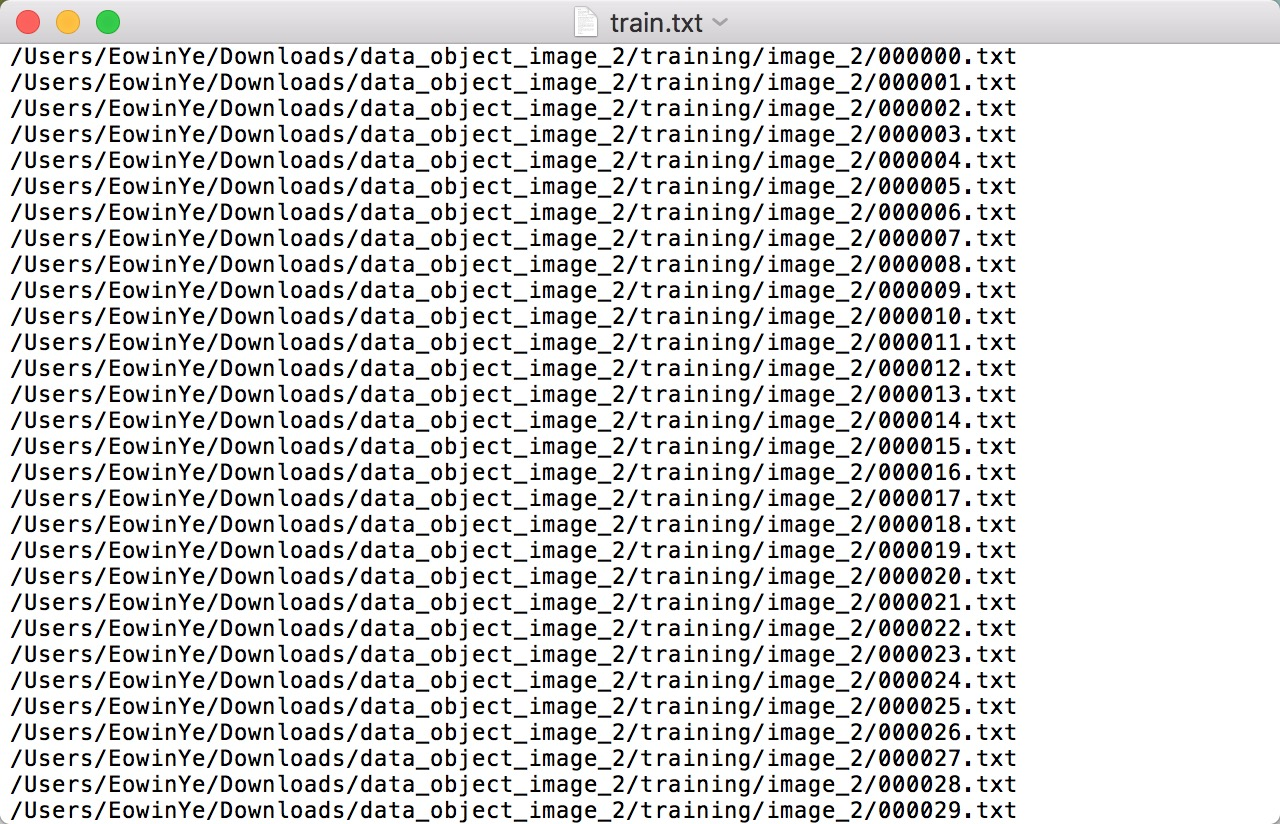
\includegraphics[width=5in]{images/trainList.png}
	\caption{Darknet标签}
	\label{trainList}
	\end{figure}
	然后,我们需要生存可以供Darknet读入的train\_list和test\_list,如图\ref{trainList}。这里直接将图片的前7000张作为训练图片,后480张作为测试图片然后生成对应的list文件即可。
}

\section{网络结构}{
网络结构参考YOLO的网络结构,在前面的章节我们已经讨论过YOLO的关键技术,这一节将主要讨论具体实现过程中的网络结构选择。

\subsection{损失函数}{
	损失函数是使用的平方误差。

	我们优化了模型输出中的平方误差。我们使用平方误差,因为它很容易优化,但是它不能完全符合我们的最大化平均精度的目标。我们增加了边界框坐标预测的损失,并减少了对不包含对象的框的置信预测的损失。我们使用两个参数,$\lambda_{coord}$和$\lambda_{noobj}$来完成这个。我们设置$\lambda_{coord}=5$和$\lambda_{noobj}=0.5$。平方误差也平等地对待大框和小框中的误差。 我们的误差度量应该反映出,大框中的小偏差比小框小。为了部分解决这个问题,我们直接预测边界框宽度和高度的平方根,而不是宽度和高度。

	在训练期间,我们优化以下多部分损失函数:
	\begin{eqnarray*}
	\lambda_{coord} \sum_{i=0}^{S^2} \sum_{j=0}^B 1_{ij}^{obj} (x_i - \hat{x_i})^2 + (y_i - \hat{y_i})^2 \\
	+ \lambda_{coord} \sum_{i=0}^{S^2} \sum_{j=0}^B 1_{ij}^{obj} (\sqrt{w_i} - \sqrt{\hat{w_i}})^2 + (\sqrt{h_i} - \sqrt{\hat{h_i}})^2 \\
	+ \sum_{i=0}^{S^2} \sum_{j=0}^B 1_{ij}^{obj} (C_i - \hat{C_i})^2 \\
	+ \lambda_{noobj} \sum_{i=0}^{S^2} \sum_{j=0}^B 1_{ij}^{noobj} (C_i - \hat{C_i})^2 \\
	+ \sum_{i=0}^{S^2} 1_{i}^{obj} \sum_{c \in classes} (p_i(c) - \hat{p_i}(c))^2
	\end{eqnarray*}

	其中$1_i^{obj}$表示如果对象出现在单元i中,并且$1_{ij}^{obj}$表示单元i中的第j个边界框预测器对于该预测是“负责的”。如果对象存在于该网格单元中,损失函数只会惩罚分类错误。 如果该预测因子对于真值框是“负责的”,则它也只对边界框坐标误差进行估计(即具有该网格单元中的任何预测变量的最高IOU)。
}

\subsection{完整网络结构YOLO}{
	\begin{figure}[htbp]
	\centering
	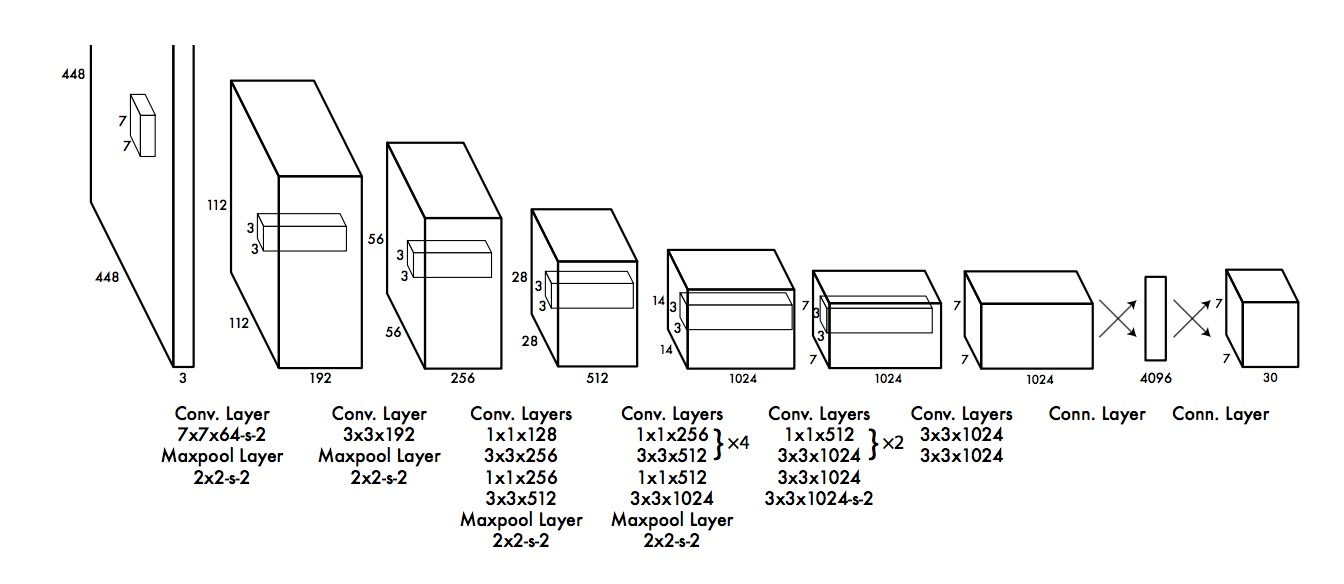
\includegraphics[width=5in]{images/net.png}
	\caption{完整网络结构YOLO}
	\label{net}
	\end{figure}
	如图\ref{net},参考YOLO和GoogLeNet模型\cite{},我们的网络有24个卷积层,其次是2个全连接层。部分卷积层后还连接了一些1*1的还原层。最后的卷积层使用了40个滤波器(num=5 * (class=3 + coords=4 + bias\_match=1))。除开最终层使用了线性激活函数,所有层使用以下leaky激活函数\ref{leaky}:
	\begin{figure}[htbp]
	\centering
	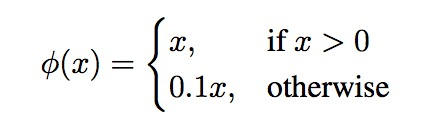
\includegraphics[width=5in]{images/leaky.png}
	\caption{leaky激活函数}
	\label{leaky}
	\end{figure}

	该网络比较大,实际训练过程中所需显存较多,训练出来的模型参数更多,理论上效果也会更好,不过速度会偏慢。
}

\subsection{缩小网络结构tiny-YOLO}{
	针对速度的要求,我们又采用了一种tiny-YOLO的网络来进行试验。

	tiny-YOLO仅有9个卷积层,并且每个卷积层使用了更少的滤波器(输出的特征),其它网络结构和之前的网络结构一样。理论上来说,tiny-YOLO将实现非常快速度的检测,同时模型大小也将降低不少,不过将造成部分精度的损失。
}
}

\section{验证方法}{
	本项目将采用计算各个类别的AP(Average Precision)的方法实现对检测结果的评估\cite{}。

	\begin{figure}[htbp]
	\centering
	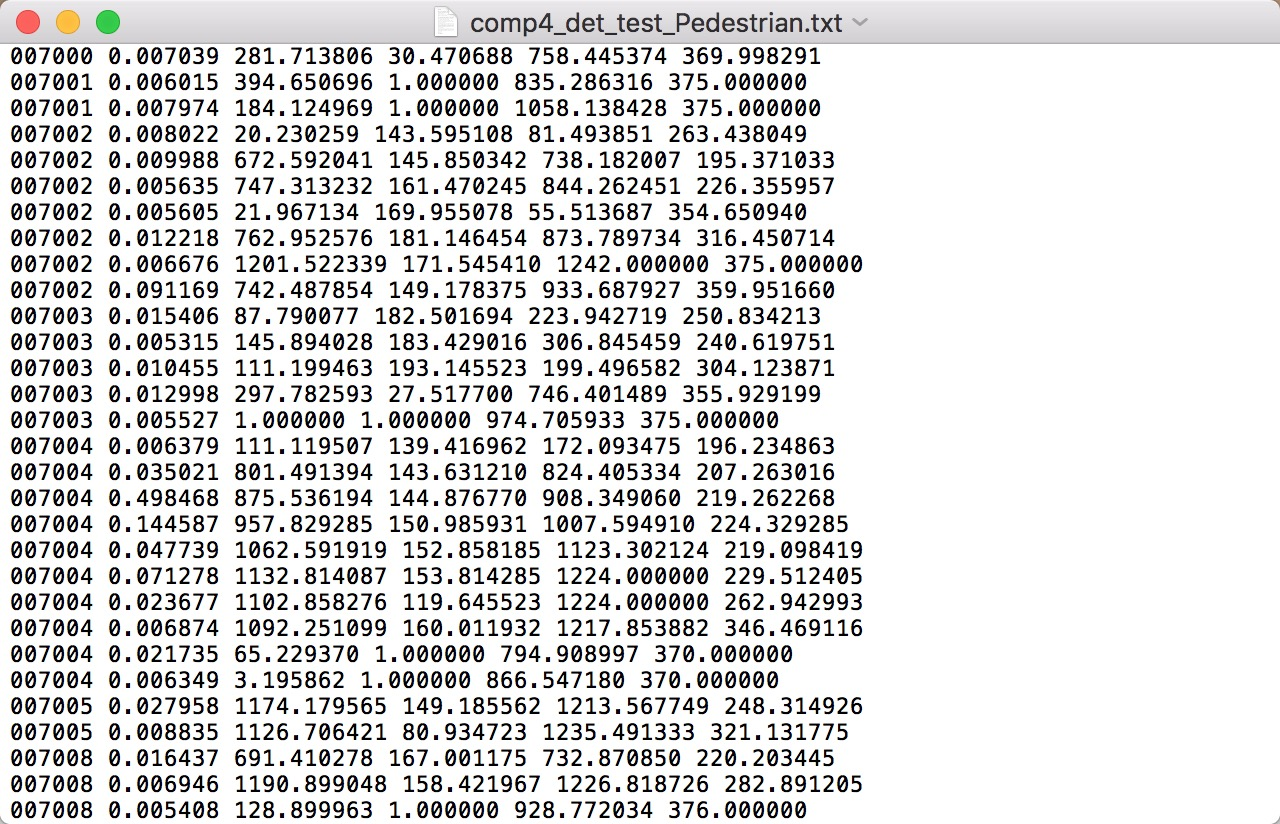
\includegraphics[width=5in]{images/results.png}
	\caption{行人验证结果}
	\label{results}
	\end{figure}
	训练好的模型对于每张图片会返回各个框的检测结果(x,y,w,h,class,precision)。而在实际验证中,每个类别会返回所有大于阈值的检测结果,如图\ref{results}。每种类都有单独的文件存放检测结果,文件形式为(img\_id, Xmin, Ymin, Xmax, Ymax, score)。我们就需要用这个检测结果和原标签对比,得到最终的实验结果。

	对于每个类,AP的具体算法如下:

	1.按照预测结果的score将预测结果按降序排序。

	2.对于每个预测结果$(\hat{X}_{min},\hat{Y}_{min},\hat{X}_{max},\hat{Y}_{max})$,找到所对应的文件中该类的各个真值$({X}_{imin},{Y}_{imin},{X}_{imax},{Y}_{imax})$,计算覆盖量IOU

	$$intersection = (max(\hat{X}_{min},{X}_{imin}) - min(\hat{X}_{max},{X}_{imax})) * (max(\hat{Y}_{min},{Y}_{imin}) - min(\hat{Y}_{max},{Y}_{imax}))$$

	$$union = (\hat{X}_{max} - \hat{X}_{min}) * (\hat{Y}_{max} - \hat{Y}_{min}) + ({X}_{imax} - {X}_{imin}) * ({Y}_{imax} - {Y}_{imin}) - intersection$$

	$$IOU = union / intersection$$

	3.更新TP(true positive),FP(false positive):选取匹配的真值中IOU最高的IOU。如果IOU大于阈值(0.5)并且该真值没有被检测到过TP就加一,否则FP加一。

	4.计算AP值:做出PR曲线,找到score降序的数组中,所有TP加一的位置,然后将这些位置i乘以前i个预测的准确率,再求和
	$$AP = \sum_{IOU>thresh}1*pre(i) / N$$其中N是真值的数量。
}

\section{本章小结}{
	本章主要讲述了本项目的整体研究流程。首先从数据集的处理上分析了KITTI数据集的特征,以及转换成YOLO所需的格式的数据预处理等;接着,我们讨论了该项目网络的损失函数,分析了所使用的各种网络结构;最后,我们讨论了测试结构的格式以及相对应的验证方法AP。
}

